\documentclass{beamer}




\usepackage{graphicx}
\usepackage{subfigure}
\usepackage{amssymb}
\usepackage{amsmath}
\usepackage{booktabs}
\usepackage{subfigure,pgf,tikz}
\usetikzlibrary{arrows}
\usepackage[misc]{ifsym}
\usepackage{mathrsfs}
\usepackage{epstopdf}
\usepackage{multicol}

\usepackage{graphicx,xcolor,subfigure}

\usepackage{xeCJK}

\setCJKmainfont{微軟正黑體}

\XeTeXlinebreaklocale "zh"

\XeTeXlinebreakskip = 0pt plus 1pt


\usetheme{Boadilla}

\setbeamertemplate{footlines}[page number]{}
\setbeamertemplate{navigation symbols}

\title[]{Hamiltonicity in locally $1$-tough graphs}

\author[]{ }



\date[]{}

\setbeamertemplate{theorems}[numbered]

\theoremstyle{plain}
\newtheorem{thm}{Theorem}[section]
\newtheorem{cor}[thm]{Corollary}
\newtheorem{lem}[thm]{Lemma}
\newtheorem{prop}[thm]{Proposition}





\theoremstyle{definition}
\newtheorem{ex}[thm]{Exercise}
\newtheorem{defn}[thm]{Definition}
\newtheorem{prob}[thm]{Problem}
\newtheorem{exam}[thm]{Example}
\newtheorem{rem}[thm]{Remark}
\newtheorem{ques}[thm]{Question}
\newtheorem{conj}[thm]{Conjecture}

\begin{document}

\begin{frame}{\bf Hamiltonian graphs}

A graph is \textcolor{red}{\bf Hamiltonian} if it contains a spanning cycle.
\bigskip


\begin{center}
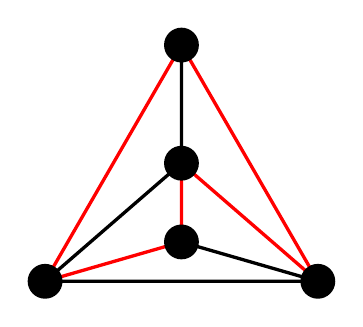
\begin{tikzpicture}[scale=2]

\foreach \i in {0,1,...,2}
{
\coordinate (v\i) at ({sin(2*\i*pi /3 r)},{cos(2*\i*pi /3 r)}) ;
}

\coordinate (v3) at (0,1/4);
\coordinate (v4) at (0,-1/4);

\draw[very thick] (v0)--(v3)--(v2)--(v1)--(v4);
\draw[very thick,color=red] (v0)--(v1)--(v3)--(v4)--(v2)--(v0);
\draw[very thick,fill] (v0) circle (.1);
\draw[very thick,fill] (v1) circle (.1);
\draw[very thick,fill] (v2) circle (.1);
\draw[very thick,fill] (v3) circle (.1);
\draw[very thick,fill] (v4) circle (.1);
\end{tikzpicture}
\bigskip

The red edges form a spanning cycle of the above graph
\end{center}
\end{frame}


\begin{frame}{\bf Definitions}


\begin{enumerate}
\item A \textcolor{red}{\bf triangulated graph} is a planar graph such that any edge is in a cycle and any face is a  triangle.
\item A \textcolor{red}{\bf chordal graph} is a graph such that every cycle of length at least $4$ contains a \textcolor{red}{\bf chord}, i.e., an edge connecting two nonadjacent vertices of the cycle.
\end{enumerate}



\begin{center}
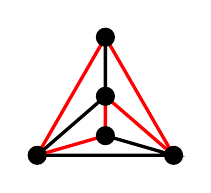
\begin{tikzpicture}[scale=1]

\foreach \i in {0,1,...,2}
{
\coordinate (v\i) at ({sin(2*\i*pi /3 r)},{cos(2*\i*pi /3 r)}) ;
}

\coordinate (v3) at (0,1/4);
\coordinate (v4) at (0,-1/4);

\draw[very thick] (v0)--(v3)--(v2)--(v1)--(v4);
\draw[very thick,color=red] (v0)--(v1)--(v3)--(v4)--(v2)--(v0);
\draw[very thick,fill] (v0) circle (.1);
\draw[very thick,fill] (v1) circle (.1);
\draw[very thick,fill] (v2) circle (.1);
\draw[very thick,fill] (v3) circle (.1);
\draw[very thick,fill] (v4) circle (.1);
\end{tikzpicture}
\end{center}
\end{frame}


\begin{frame}
\begin{rem} 
\begin{enumerate}
\item A triangulated of order at least $4$ contains $3+3(n-3)=3n-6$ edges and $2n-4$ faces.
\item If $C$ is a Hamiltonian cycle of a triangulated planar graph $T$ then there are $n-2$ faces and $n-3$ edges inside $C$. 
\end{enumerate}
\end{rem}
\end{frame}

\begin{frame}{\bf Problem}

Can every edge of a triangulated graph be drawn as an edge of an outer face.
\bigskip


{\bf Answer:} Yes


\bigskip

\begin{center}
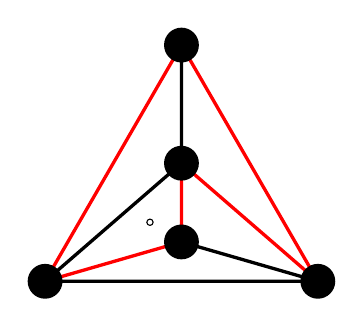
\begin{tikzpicture}[scale=2]

\foreach \i in {0,1,...,2}
{
\coordinate (v\i) at ({sin(2*\i*pi /3 r)},{cos(2*\i*pi /3 r)}) ;
}

\coordinate (v3) at (0,1/4);
\coordinate (v4) at (0,-1/4);

\draw[very thick] (v0)--(v3)--(v2)--(v1)--(v4);
\draw[very thick,color=red] (v0)--(v1)--(v3)--(v4)--(v2)--(v0);
\draw[very thick,fill] (v0) circle (.1);
\draw[very thick,fill] (v1) circle (.1);
\draw[very thick,fill] (v2) circle (.1);
\draw[very thick,fill] (v3) circle (.1);
\draw[very thick,fill] (v4) circle (.1);
\draw[] (-1/5, -1/8) circle (.02);
\end{tikzpicture}
\end{center}
\bigskip


Plane is homeomorphic to the surface obtained from a sphere deleting a point.
\end{frame}




\begin{frame}{\bf A $4$-regular triangulated graph}

\begin{center}
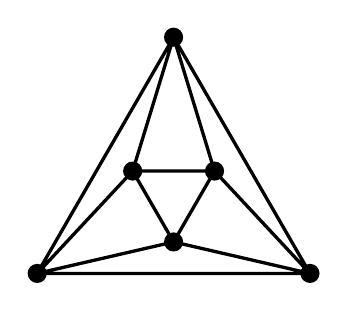
\begin{tikzpicture}[scale=1]

\foreach \i in {0,1,2}
{
\coordinate (v\i) at ({2*sin(2*\i*pi /3 r)},{2*cos(2*\i*pi /3 r)}) ;
}

\foreach \i in {3,4,5}
{
\coordinate (v\i) at ({0.6*sin(2*(2*\i-5)*pi /6 r)},{0.6*cos(2*(2*\i-5)*pi /6 r)}) ;
}



\draw[very thick]    (v0)--(v1)--(v2)--(v0) (v3)--(v4)--(v5)--(v3) (v0)--(v3)--(v1)--(v4)--(v2)--(v5)--(v0);
\draw[very thick,fill] (v0) circle (.1);
\draw[very thick,fill] (v1) circle (.1);
\draw[very thick,fill] (v2) circle (.1);
\draw[very thick,fill] (v3) circle (.1);
\draw[very thick,fill] (v4) circle (.1);
\draw[very thick,fill] (v5) circle (.1);
\end{tikzpicture}
\end{center}

\end{frame}


\begin{frame}{\bf A triangulated graph which is not a chordal graph}

\begin{center}
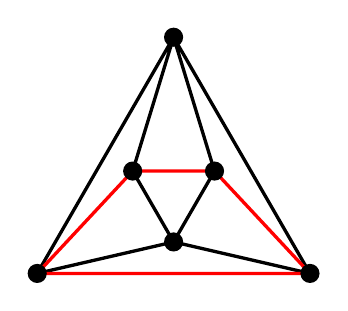
\begin{tikzpicture}[scale=1]

\foreach \i in {0,1,2}
{
\coordinate (v\i) at ({2*sin(2*\i*pi /3 r)},{2*cos(2*\i*pi /3 r)}) ;
}

\foreach \i in {3,4,5}
{
\coordinate (v\i) at ({0.6*sin(2*(2*\i-5)*pi /6 r)},{0.6*cos(2*(2*\i-5)*pi /6 r)}) ;
}



\draw[very thick]    (v0)--(v1)--(v4) (v2)--(v0) (v3)--(v4)--(v5)--(v0)--(v3)--(v4)--(v2) ;
\draw[very thick, color=red] (v3)--(v1)--(v2)--(v5)--(v3);
\draw[very thick,fill] (v0) circle (.1);
\draw[very thick,fill] (v1) circle (.1);
\draw[very thick,fill] (v2) circle (.1);
\draw[very thick,fill] (v3) circle (.1);
\draw[very thick,fill] (v4) circle (.1);
\draw[very thick,fill] (v5) circle (.1);
\end{tikzpicture}



There is no chord in the red cycle.
\end{center}
\end{frame}


\begin{frame}{\bf More definitions}
\begin{enumerate}
\item A \textcolor{red}{\bf weakly  pancyclic graph} is a graph which contains cycles of every length between the girth and the circumference.
\item A graph is \textcolor{red}{\bf $t$-tough}  if for every integer $k>1$, the graph cannot be split into $k$ components by removal of fewer than $tk$ vertices
\item The \textcolor{red}{\bf toughness} a non-complete graph $G$ is the maximum $t$ such that $G$ is $t$-tough. The toughness of a complete graph is $\infty$.
\end{enumerate}

\begin{center}
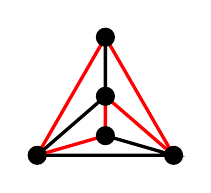
\begin{tikzpicture}[scale=1]

\foreach \i in {0,1,...,2}
{
\coordinate (v\i) at ({sin(2*\i*pi /3 r)},{cos(2*\i*pi /3 r)}) ;
}

\coordinate (v3) at (0,1/4);
\coordinate (v4) at (0,-1/4);

\draw[very thick] (v0)--(v3)--(v2)--(v1)--(v4);
\draw[very thick,color=red] (v0)--(v1)--(v3)--(v4)--(v2)--(v0);
\draw[very thick,fill] (v0) circle (.1);
\draw[very thick,fill] (v1) circle (.1);
\draw[very thick,fill] (v2) circle (.1);
\draw[very thick,fill] (v3) circle (.1);
\draw[very thick,fill] (v4) circle (.1);
\end{tikzpicture}
\end{center}

\begin{rem}
A $t$-tough graph with $t>0$ is connected and  a Hamiltonian graph is $1$-tough.
\end{rem}
\end{frame}




\begin{frame}{\bf A triangulated graph which is not weakly pancyclic}

To be filled later. 
\end{frame}



\begin{frame}{\bf A long standing conjecture}

There is a positive constant $t$ such that every $t$-tough graph is Hamiltonian.
\bigskip

V. Chv\'{a}tal, Tough graphs and hamiltonian circuits, Discrete Math. 5 (1973), 215-228.

\end{frame}













\begin{frame}{\bf Locally property $P$}

Let $P$ be a property on graphs.
A graph $G$ has \textcolor{red}{\bf local $P$} if $G_1(v)$ has property $P$ for every vertex $v$ in $G$.
\bigskip




\begin{center}
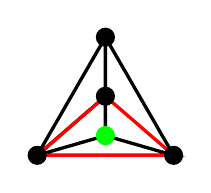
\begin{tikzpicture}[scale=1]

\foreach \i in {0,1,...,2}
{
\coordinate (v\i) at ({sin(2*\i*pi /3 r)},{cos(2*\i*pi /3 r)}) ;
}

\coordinate (v3) at (0,1/4);
\coordinate (v4) at (0,-1/4);

\draw[very thick] (v1)--(v0)--(v3)--(v2)--(v1)--(v4)--(v2)--(v0) (v3)--(v4) ;
\draw[very thick,color=red] (v1)--(v3)--(v2)--(v1);
\draw[very thick,fill] (v0) circle (.1);
\draw[very thick,fill] (v1) circle (.1);
\draw[very thick,fill] (v2) circle (.1);
\draw[very thick,fill] (v3) circle (.1);
\draw[very thick,fill, color=green] (v4) circle (.1);
\end{tikzpicture}
\end{center}
\bigskip


\begin{rem}
A triangulated graph of order at least $4$ is locally Hamiltonian.
\end{rem}
\end{frame}


\begin{frame}{\bf A $1$-tough and locally connected planar graph}
\begin{center}
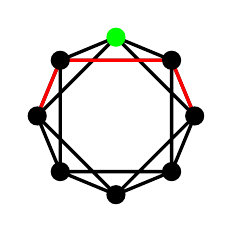
\begin{tikzpicture}[scale=1]

\foreach \i in {0,1,...,7}
{
\coordinate (v\i) at ({sin(2*\i*pi /8 r)},{cos(2*\i*pi /8 r)}) ;
}


\draw[very thick] (v0)--(v1)--(v2)--(v3)--(v4)--(v5)--(v6)--(v7)--(v0)--(v2)--(v4)--(v6)--(v0) (v1)--(v3)--(v5)--(v7)--(v1);
\draw[very thick,color=red] (v6)--(v7)--(v1)--(v2);
\draw[very thick,fill, color=green] (v0) circle (.1);
\draw[very thick,fill] (v1) circle (.1);
\draw[very thick,fill] (v2) circle (.1);
\draw[very thick,fill] (v3) circle (.1);
\draw[very thick,fill] (v4) circle (.1);
\draw[very thick,fill] (v5) circle (.1);
\draw[very thick,fill] (v6) circle (.1);
\draw[very thick,fill] (v7) circle (.1);
\end{tikzpicture}
\end{center}
\bigskip


The planar graph $DL(8;1,2)$ is $1$-tough and locally connected.
\bigskip



\begin{rem}
$DL(n;1, 2)$ is a planar graph, where $n\geq 4$ and $n$ is even.
\end{rem}



\begin{rem}
Every planar graph can be drawn by using straight lines as edges.
\end{rem}
\end{frame}


\begin{frame}{\bf Question}

Is a triangulated graph $1$-tough?
\bigskip

The answer is `no' as shown in the next page.

\end{frame}

\begin{frame}{\bf A triangulated graph which is not $1$-tough}

\begin{center}
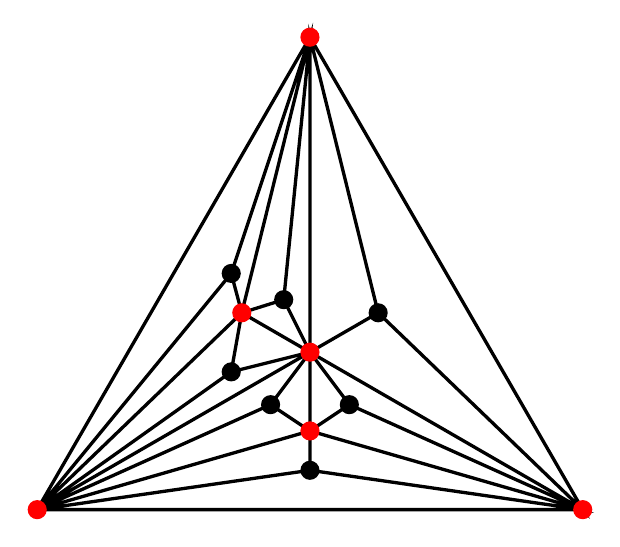
\begin{tikzpicture}[scale=1]

\foreach \i in {0,1,2}
{
\coordinate (v\i) at ({4*sin(2*\i*pi /3 r)},{4
*cos(2*\i*pi /3 r)}) ;
}

\foreach \i in {3,4,5}
{
\coordinate (v\i) at ({sin(2*(2*\i-5)*pi /6 r)},{cos(2*(2*\i-5)*pi /6 r)}) ;
}


\coordinate (v6) at (0,0);
\coordinate (v7) at (1/2,-2/3);
\coordinate (v8) at (0,-3/2);
\coordinate (v9) at (-1/2,-2/3);
\coordinate (v10) at (-1/3,2/3);
\coordinate (v11) at (-1,-1/4);
\coordinate (v12) at (-1,1);


\draw[very thick] (v3)--(v0)--(v6)--(v1)--(v2)--(v0)   (v8)--(v2)--(v6)--(v5)--(v11)  (v7)--(v4)--(v1)--(v3) (v0)--(v1)--(v3)--(v6)--(v4)--(v2)--(v5)--(v0)
(v4)--(v8)--(v1)--(v7)--(v6)  (v4)--(v9)--(v6)  (v9)--(v2)--(v12) (v6)--(v10)--(v0)--(v12)--(v5)  (v10)--(v5)--(v11)--(v6) (v11)--(v2);

\draw[very thick,fill, color=red] (v0) circle (.1);
\draw[very thick,fill,  color=red] (v1) circle (.1);
\draw[very thick,fill, color=red] (v2) circle (.1);
\draw[very thick,fill] (v3) circle (.1);
\draw[very thick,fill, color=red] (v4) circle (.1);
\draw[very thick,fill, color=red] (v5) circle (.1);
\draw[very thick,fill, color=red] (v6) circle (.1);
\draw[very thick,fill] (v7) circle (.1);
\draw[very thick,fill] (v8) circle (.1);
\draw[very thick,fill] (v9) circle (.1);
\draw[very thick,fill] (v10) circle (.1);
\draw[very thick,fill] (v11) circle (.1);
\draw[very thick,fill] (v12) circle (.1);
\end{tikzpicture}
\bigskip

Deleting the $6$ red vertices will yield $7$ components.

\end{center}

\end{frame}


\begin{frame}{\bf Lemma}
For a vertex $u$ and  a cut set $S$ of $G$ if $c(G-S)> |S|$ and $G-u$ is $1$-tough
then $u\not\in S$ and $G_1(u)\subseteq S$.
\bigskip

\begin{proof}
If $u\in S$ then $G-u$ has toughness at most $(|S|-1)/c(G-S)<1$, a contradiction;
if $u\not\in S$ then $G-u$ being $1$-tough and $|S|/c(G-S)<1$
implies that there is a single element component $\{u\}$ in $G-S$, so $G_1(u)\subseteq S$.
\end{proof}
\bigskip


T. Nishizeki, A $1$-tough nonhamiltonian maximal planar graph, Discrete Math. 30(1980), 305-307.
\end{frame}


\begin{frame}{\bf Proposition} 
Let $G$ be a connected graph such that  $G-u$ is Hamiltonian for every vertex in $G$.  Then $G$ is $1$-tough. 
\begin{proof}
Suppose $G$ is not $1$-tough and pick a cut set $S$ with $c(G-S)> |S|$. 
As $G-u$  is $1$-tough, $u\not\in S$ by previous lemma. Hence $S=\emptyset,$ a contradiction. 
\end{proof}

\end{frame}

\begin{frame}{\bf Question}

Is every $1$-tough and  locally connected graph Hamiltonian?


\end{frame}


\begin{frame}{\bf A $1$-tough, locally connected, non-Hamiltonian planar graph}
\begin{center}
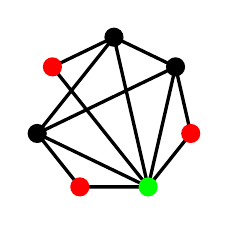
\begin{tikzpicture}[scale=1]

\foreach \i in {0,1,...,6}
{
\coordinate (v\i) at ({sin(2*\i*pi /7 r)},{cos(2*\i*pi /7 r)}) ;
}


\draw[very thick] (v0)--(v1)--(v2)--(v3)--(v4)--(v5)--(v0)--(v3) (v1)--(v5)  (v3)--(v6)--(v0)  (v5)--(v3)--(v1) ;
\draw[very thick,fill] (v0) circle (.1);
\draw[very thick,fill] (v1) circle (.1);
\draw[very thick,fill, color=red] (v2) circle (.1);
\draw[very thick,fill, color=green] (v3) circle (.1);
\draw[very thick,fill, color=red] (v4) circle (.1);
\draw[very thick,fill] (v5) circle (.1);
\draw[very thick,fill, color=red] (v6) circle (.1);
\end{tikzpicture}
\end{center}


\bigskip


The graph is not Hamiltonian since the two edges of  each red vertex are in every Hamiltonian cycle.

\end{frame}




\begin{frame}{\bf A $1$-tough and locally Hamiltonian planar graph}


\begin{multicols}{2}


\begin{center}
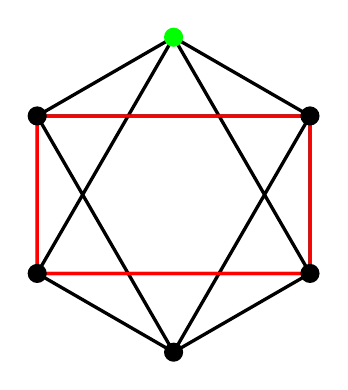
\begin{tikzpicture}[scale=1]

\foreach \i in {0,1,...,5}
{
\coordinate (v\i) at ({2*sin(2*\i*pi /6 r)},{2*cos(2*\i*pi /6 r)}) ;
}


\draw[very thick] (v4)--(v2)--(v0)--(v1)--(v2)--(v3)--(v4)--(v5)--(v0)--(v4) (v5)--(v3)--(v1)--(v5) ;
\draw[very thick,color=red] (v1)--(v2)--(v4)--(v5)--(v1);
\draw[very thick,fill,  color=green] (v0) circle (.1);
\draw[very thick,fill] (v1) circle (.1);
\draw[very thick,fill] (v2) circle (.1);
\draw[very thick,fill] (v3) circle (.1);
\draw[very thick,fill] (v4) circle (.1);
\draw[very thick,fill] (v5) circle (.1);
\end{tikzpicture}
\end{center}
\bigskip


\begin{center}
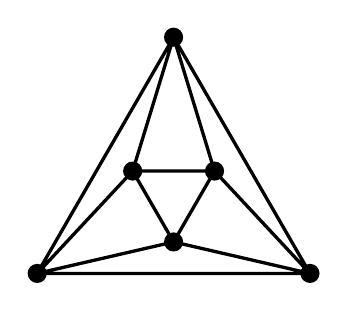
\begin{tikzpicture}[scale=1]

\foreach \i in {0,1,2}
{
\coordinate (v\i) at ({2*sin(2*\i*pi /3 r)},{2*cos(2*\i*pi /3 r)}) ;
}

\foreach \i in {3,4,5}
{
\coordinate (v\i) at ({0.6*sin(2*(2*\i-5)*pi /6 r)},{0.6*cos(2*(2*\i-5)*pi /6 r)}) ;
}



\draw[very thick]    (v0)--(v1)--(v2)--(v0) (v3)--(v4)--(v5)--(v3) (v0)--(v3)--(v1)--(v4)--(v2)--(v5)--(v0);
\draw[very thick,fill] (v0) circle (.1);
\draw[very thick,fill] (v1) circle (.1);
\draw[very thick,fill] (v2) circle (.1);
\draw[very thick,fill] (v3) circle (.1);
\draw[very thick,fill] (v4) circle (.1);
\draw[very thick,fill] (v5) circle (.1);
\end{tikzpicture}
\end{center}

\end{multicols}

The planar  graph $DL(6;1,2)$ is $1$-tough and locally Hamiltonian, implying locally $1$-tough.
$DL(6;1,2)$ is  a triangulated planar graph.
\bigskip




\end{frame}


\begin{frame}{\bf Question}

Is every $1$-tough and locally $1$-tough graph locally Hamiltonian?
\bigskip


The answer is `no' in the following page.

\end{frame}

\begin{frame}{\bf A $1$-tough and locally $1$-tough graph \\
which is not locally Hamiltonian}
\begin{center}
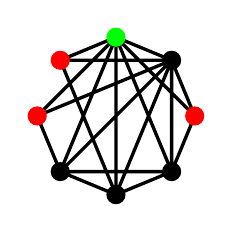
\begin{tikzpicture}[scale=1]

\foreach \i in {0,1,...,7}
{
\coordinate (v\i) at ({sin(2*\i*pi /8 r)},{cos(2*\i*pi /8 r)}) ;
}


\draw[very thick] (v3)--(v0)--(v1)--(v2)--(v3)--(v4)--(v5)--(v6) (v7)--(v0)--(v2)  (v1)--(v5)--(v0)--(v4)  (v0)--(v6)--(v1)--(v7)--(v4) (v3)--(v5) (v3)--(v1)--(v4);
\draw[very thick,fill, color=green] (v0) circle (.1);
\draw[very thick,fill] (v1) circle (.1);
\draw[very thick,fill, color=red] (v2) circle (.1);
\draw[very thick,fill] (v3) circle (.1);
\draw[very thick,fill] (v4) circle (.1);
\draw[very thick,fill] (v5) circle (.1);
\draw[very thick,fill, color=red] (v6) circle (.1);
\draw[very thick,fill, color=red] (v7) circle (.1);
\end{tikzpicture}
\end{center}
\bigskip


Deleting the green vertex of the above graph yields a $1$-tough non-Hamiltonian graph (The red vertices have degree $2$).

\bigskip

The above graph is not planar.

\end{frame}


\begin{frame}{\bf Question}

Is a $1$-tough and locally $1$-tough graph Hamiltonian.

\bigskip

The answer is `no' as shown in the next page.

\end{frame}


\begin{frame}{\bf A triangulated $1$-tough non-Hamiltonian graph }

\begin{center}
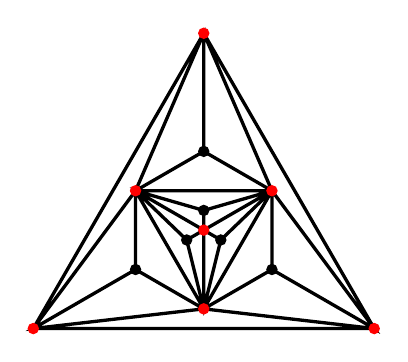
\begin{tikzpicture}[scale=0.5]

\foreach \i in {0,1,2}
{
\coordinate (v\i) at ({5*sin(2*\i*pi /3 r)},{5
*cos(2*\i*pi /3 r)}) ;
}

\foreach \i in {3,4,5,6,7,8}
{
\coordinate (v\i) at ({2*sin(2*(\i-3)*pi /6 r)},{2*cos(2*(\i-3)*pi /6 r)}) ;
}


\foreach \i in {9,10, 11}
{
\coordinate (v\i) at ({0.5*sin(2*(\i-9)*pi /3 r)},{0.5*cos(2*(\i-9)*pi /3 r)}) ;
}

\coordinate (v12) at (0,0);


\draw[very thick] (v4)--(v9)--(v8)--(v11)--(v6)--(v10)--(v4)--(v8)--(v6)--(v4)--(v0)--(v1)--(v2)--(v0)--(v3)--(v4)--(v5)--(v6)--(v7)--(v8)--(v3)
(v4)--(v1)--(v5) (v7)--(v2)--(v6)--(v1) (v2)--(v8) (v10)--(v12)--(v9) (v4)--(v12)--(v11) (v6)--(v12)--(v8)--(v0);

\draw[very thick,fill, color=red] (v0) circle (.1);
\draw[very thick,fill,  color=red] (v1) circle (.1);
\draw[very thick,fill, color=red] (v2) circle (.1);
\draw[very thick,fill] (v3) circle (.1);
\draw[very thick,fill, color=red] (v4) circle (.1);
\draw[very thick,fill] (v5) circle (.1);
\draw[very thick,fill, color=red] (v6) circle (.1);
\draw[very thick,fill] (v7) circle (.1);
\draw[very thick,fill, color=red] (v8) circle (.1);
\draw[very thick,fill] (v9) circle (.1);
\draw[very thick,fill] (v10) circle (.1);
\draw[very thick,fill] (v11) circle (.1);
\draw[very thick,fill,, color=red] (v12) circle (.1);
\end{tikzpicture}

Seven separating triangles in the above graph.

\end{center}
\bigskip



Michal Tk\'{a}\v{c}, On the shortness exponent of l-tough, maximal planar graphs, Discrete Math. 154(1996), 321-328.
\end{frame}







\begin{frame}{\bf Plan}

We shall develop theory of  $1$-tough and locally $1$-tough graph.

\end{frame}







\begin{frame}{\bf Lemma}
If $G$ is $1$-tough and locally $1$-tough then $G-u$ is $1$-tough for every vertex $u$ in $G$.

\begin{proof}
Assume that $G-u$ is not $1$-tough. Then $G-u$ is split into $k\geq 2$ components by removal of some subset $S$ of vertices with $|S|<k$, where $u\not\in S$. Assume $\ell$ of these $k$ components intersecting with $G_1(u)$. If $\ell=1$ then by connecting $u$ to this unique component intersecting with $G_1(u)$, there are $k$ components after removal of $S$ from $G$, a contradiction to the $1$-tough property of $G$.
\medskip

Assume $\ell\geq 2$. Then  $|S\cap G_1(u)|\geq \ell$ since $G_1(u)$ is $1$-tough.
Similarly by connecting $u$ to these $\ell$ components intersecting with $G_1(u)$ to form a component, we find $k-\ell+1$ components
after the removal of $S-G_1(u)$ from $G$.  Hence $|S-G_1(u)|\geq k-\ell+1$ since $G$ is $1$-tough.
Then $S=|S\cap G_1(u)|+|S-G_1(u)|\geq \ell+(k-\ell+1)=k+1$, a contradiction.
\end{proof}

\end{frame}


\begin{frame}{\bf Lemma}
If $G$ is $1$-tough and locally $1$-tough then $G$ has toughness greater than $1$.

\begin{proof}
Assume that $G$ has toughness $1$ and pick a subset $S$ of $k$ vertices whose removal will yield $k$ components. Pick $u$ in $S$.
Then the removal of $k-1$ vertices in $S-\{u\}$ from $G-u$ will yield $k$ components, a contradiction to $G-u$ being $1$-tough by previous lemma.
\end{proof}
\end{frame}

\begin{frame}{\bf Toughness of a $1$-tough and locally $1$-tough graph}

By connecting a new vertex to the complete bipartite graph $K_{t, t}$, we have a $1$-tough and locally $1$-tough graph with toughness $(t+1)/t$ for evert $t\geq 1$. Hence the toughness of a $1$-tough and locally $1$-tough graph can approximate to $1$.

\end{frame}


\begin{frame}{\bf Lemma}
If $G$ is $1$-tough and locally $1$-tough of order at least $4$ then $G$ has minimum degree at least $3$.
\bigskip

\begin{proof} If $G$ has minimum degree at most $2$ then $G$ has toughness at most $1=2/2$
because deleting the neighbors of a vertex with minimum degree yields at least two components.
\end{proof}


\begin{rem}
There is only one $1$-tough and locally $1$-tough graph with maximum degree $3$.
\end{rem}


\begin{center}
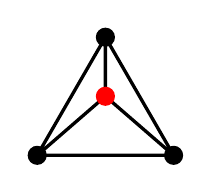
\begin{tikzpicture}[scale=1]

\foreach \i in {0,1,...,2}
{
\coordinate (v\i) at ({sin(2*\i*pi /3 r)},{cos(2*\i*pi /3 r)}) ;
}

\coordinate (v3) at (0,1/4);


\draw[very thick] (v0)--(v3)--(v2)--(v1) (v0)--(v1)--(v3)  (v2)--(v0);
\draw[very thick,fill] (v0) circle (.1);
\draw[very thick,fill] (v1) circle (.1);
\draw[very thick,fill] (v2) circle (.1);
\draw[very thick,fill, color=red] (v3) circle (.1);
\end{tikzpicture}
\end{center}

\end{frame}


\begin{frame}{\bf Lemma}
If $G$ is $1$-tough and locally $1$-tough of order at least $4$ then every edge of $G$ is in at least two triangles.
\bigskip

\begin{proof} Let $e=uv$ be an edge of $G$. Since $u$ has degree at least $3$, $G_1(u)$ is at least $3$, so with  the $1$-tough property of $G_1(u)$, $u$ has at least two neighbors in $G_1(u)$, forming two triangles containing the edge $e$.
\end{proof}
\end{frame}

\begin{frame}{\bf Each edge is in two triangles}

\begin{center}
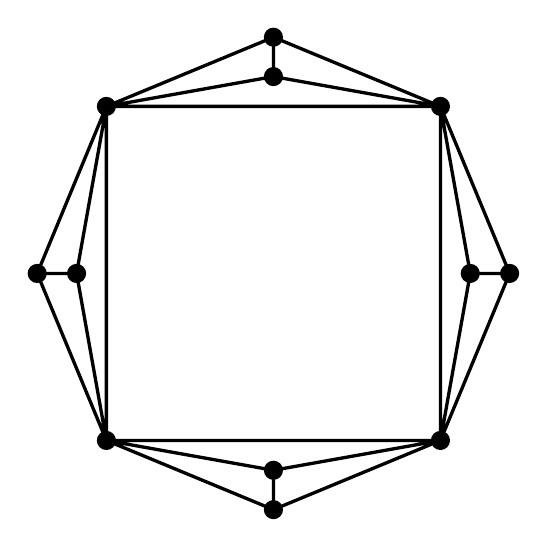
\begin{tikzpicture}[scale=1]

\foreach \i in {0,1,...,7}
{
\coordinate (v\i) at ({3*sin(2*\i*pi /8 r)},{3*cos(2*\i*pi /8 r)}) ;
}


\foreach \i in {8,9,10,11}
{
\coordinate (v\i) at ({2.5*sin(4*(\i-8)*pi /8 r)},{2.5*cos(4*(\i-8)*pi /8 r)}) ;
}


\draw[very thick] (v0)--(v1)--(v2)--(v3)--(v4)--(v5)--(v6)--(v7)--(v0) (v0)--(v8) (v2)--(v9) (v4)--(v10) (v6)--(v11)
(v1)--(v3)--(v5)--(v7)--(v1) (v8)--(v1)--(v9)--(v3)--(v10)--(v5)--(v11)--(v7)--(v8) ;
\draw[very thick,fill] (v0) circle (.1);
\draw[very thick,fill] (v1) circle (.1);
\draw[very thick,fill] (v2) circle (.1);
\draw[very thick,fill] (v3) circle (.1);
\draw[very thick,fill] (v4) circle (.1);
\draw[very thick,fill] (v5) circle (.1);
\draw[very thick,fill] (v6) circle (.1);
\draw[very thick,fill] (v7) circle (.1);
\draw[very thick,fill] (v8) circle (.1);
\draw[very thick,fill] (v9) circle (.1);
\draw[very thick,fill] (v10) circle (.1);
\draw[very thick,fill] (v11) circle (.1);
\end{tikzpicture}
\bigskip

Each edge of the above non-triangulated graph is in two triangles. This graph is $1$-tough, but not locally $1$-tough.
\end{center}


\end{frame}

\begin{frame}{\bf Proposition}
If $G$ is a $1$-tough and locally $1$-tough planar graph of order at least $4$ and $C$ is a cycle of maximum length in $G$, then
each edge in $C$ is in at least two triangles of the subgraph induced on the vertex set of $C$.
\bigskip

\begin{proof}  If the two triangles of an edge in previous lemma contain a vertex not in $C$ then we have a cycle of length one more than that of $C$, a contradiction to the maximum length assumption of $C$.
\end{proof}
\end{frame}


\begin{frame}{\bf $1$-tough and locally Hamiltonian planar graph of order $7$}


\begin{multicols}{2}


\begin{center}
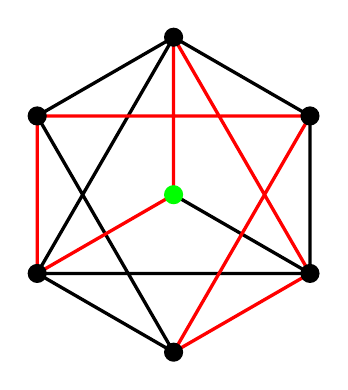
\begin{tikzpicture}[scale=1]

\foreach \i in {0,1,...,5}
{
\coordinate (v\i) at ({2*sin(2*\i*pi /6 r)},{2*cos(2*\i*pi /6 r)}) ;
}
\coordinate (v6) at (0,0);

\draw[very thick] (v3)--(v5)--(v0)--(v1)--(v2)--(v4)--(v3)  (v0)--(v4) (v2)--(v6);
\draw[very thick,color=red] (v0)--(v6)--(v4)--(v5)--(v1)--(v3)--(v2)--(v0);
\draw[very thick,fill] (v0) circle (.1);
\draw[very thick,fill] (v1) circle (.1);
\draw[very thick,fill] (v2) circle (.1);
\draw[very thick,fill] (v3) circle (.1);
\draw[very thick,fill] (v4) circle (.1);
\draw[very thick,fill] (v5) circle (.1);
\draw[very thick,fill, color=green] (v6) circle (.1);
\end{tikzpicture}




The graph $DL(6;1,2)^+$.

\end{center}
\bigskip




\begin{center}
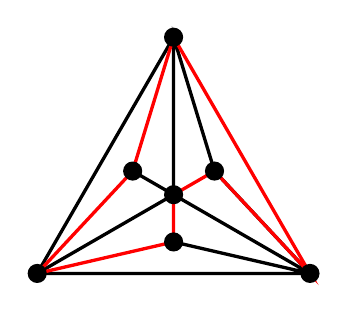
\begin{tikzpicture}[scale=1]

\foreach \i in {0,1,2}
{
\coordinate (v\i) at ({2*sin(2*\i*pi /3 r)},{2*cos(2*\i*pi /3 r)}) ;
}

\foreach \i in {3,4,5}
{
\coordinate (v\i) at ({0.6*sin(2*(2*\i-5)*pi /6 r)},{0.6*cos(2*(2*\i-5)*pi /6 r)}) ;
}

\coordinate (v6) at (0,0);

\draw[very thick] (v3)--(v0)--(v6)--(v1)--(v2)--(v0)   (v2)--(v6)--(v5) (v4)--(v1)--(v3);
\draw[very thick,color=red] (v0)--(v1)--(v3)--(v6)--(v4)--(v2)--(v5)--(v0);
\draw[very thick,fill] (v0) circle (.1);
\draw[very thick,fill] (v1) circle (.1);
\draw[very thick,fill] (v2) circle (.1);
\draw[very thick,fill] (v3) circle (.1);
\draw[very thick,fill] (v4) circle (.1);
\draw[very thick,fill] (v5) circle (.1);
\draw[very thick,fill] (v6) circle (.1);
\end{tikzpicture}

\bigskip


A triangulated graph of order $7$ (There are many different ones including $DL(6;1,2)^+$).

\end{center}
\end{multicols}


\end{frame}


\begin{frame}{\bf Problems}

\begin{enumerate}
\item For $n\leq 7$, find  non-triangulated planar Hamiltonian graphs of order $n$  such that each edge in its Hamiltonian cycle is in two triangles.
\item How many edges are possible for a planar Hamiltonian graph of order $n$ such that each edge in its Hamiltonian cycle is in two triangles?
\item Determine all the  non-triangulated planar Hamiltonian graphs of order $n$  such that each edge in its Hamiltonian cycle is in two triangles.
\item Find a $1$-tough and locally $1$-tough planar graph which is not triangulated.
\end{enumerate}
\end{frame}


\begin{frame}{\bf Lemma}
Let $S$ be a cut set of a locally $1$-tough connected graph $G$. If $x\in S$ is connected to at least two components in $G-S$ then $x$ has degree at least two in the subgraph induced on $S$.
\begin{proof}
The $1$-tough of $G_1(x)$ implies $|G_1(x)\cap S|$ is at least the number of components in $G-S$ that are connected to $x$.
\end{proof}

A cut set $S$ of $G$ is \textcolor{red}{\bf effective} if each  $x\in S$ is connected to at least two components in $G-S$.
\end{frame}


\begin{frame}{\bf Effective cut set}
\begin{center}
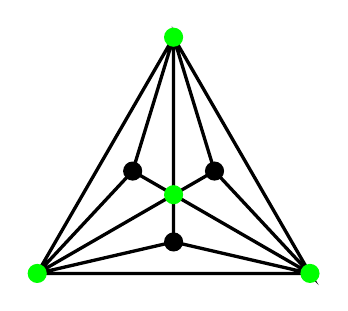
\begin{tikzpicture}[scale=1]

\foreach \i in {0,1,2}
{
\coordinate (v\i) at ({2*sin(2*\i*pi /3 r)},{2*cos(2*\i*pi /3 r)}) ;
}

\foreach \i in {3,4,5}
{
\coordinate (v\i) at ({0.6*sin(2*(2*\i-5)*pi /6 r)},{0.6*cos(2*(2*\i-5)*pi /6 r)}) ;
}

\coordinate (v6) at (0,0);

\draw[very thick] (v3)--(v0)--(v6)--(v1)--(v2)--(v0)   (v2)--(v6)--(v5) (v4)--(v1)--(v3) (v0)--(v1)--(v3)--(v6)--(v4)--(v2)--(v5)--(v0);
\draw[very thick,fill, color=green] (v0) circle (.1);
\draw[very thick,fill, color=green] (v1) circle (.1);
\draw[very thick,fill, color=green] (v2) circle (.1);
\draw[very thick,fill] (v3) circle (.1);
\draw[very thick,fill] (v4) circle (.1);
\draw[very thick,fill] (v5) circle (.1);
\draw[very thick,fill, color=green] (v6) circle (.1);
\end{tikzpicture}

\bigskip


The green vertices form an effective cut set.

\end{center}

\end{frame}
\end{document} 